In this section we try to find a model able to explain the categorical variable \textit{"TARGET\_5YRS"} through classification techniques.
In particular we are going to use 
\begin{itemize}
	\item Classification trees with ensemble methods
	\item Logistic regression
\end{itemize}

The first thing was to check if the dataset is balanced or not. In figure \Fig~\ref{fig:target_bar_plot} we can clearly see that the 1278 samples are not equally distributed. 

\begin{figure}[h]
	\centering
	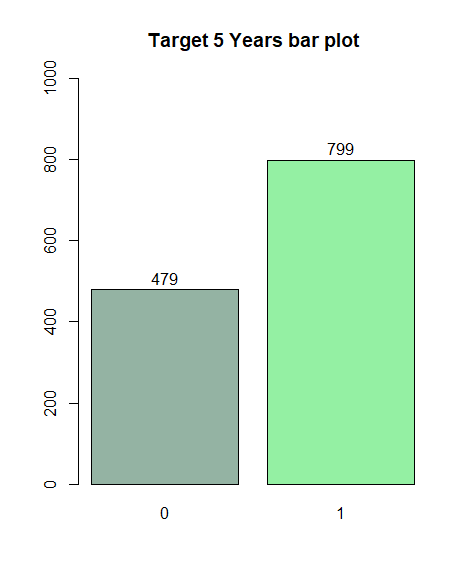
\includegraphics[width=0.5\linewidth]{ImageFiles/Classification/target_bar_plot}
	\caption{Target variable bar plot}
	\label{fig:target_bar_plot}
\end{figure}

After this, we removed two columns from the cleaned dataset because they were linerly dependent with some others
\begin{itemize}
	\item \textit{"PTS"}, linear combination of \textit{"FGM"}, \textit{"X3P\_MADE"}, and \textit{"FTM"}
	\item \textit{"REB"}, linear combination of \textit{"OREB"} and \textit{"DREB"}
\end{itemize}
